\documentclass{standalone}
\usepackage{tikz}
\usepackage{amsthm, amsfonts}

\begin{document}
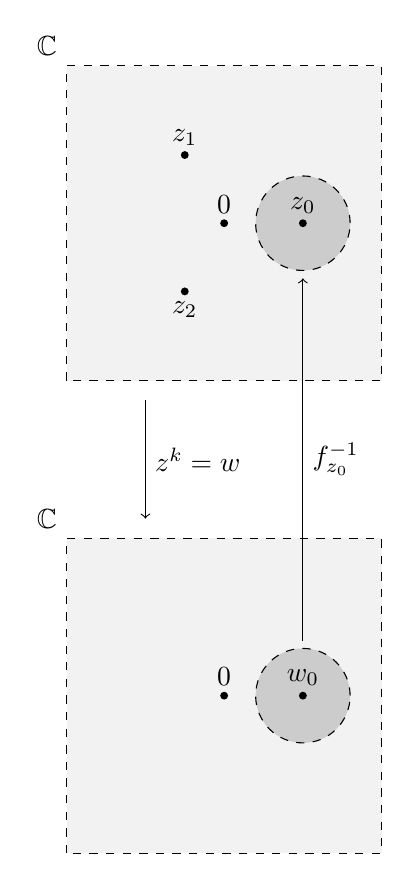
\begin{tikzpicture}
\draw (-2,2) node[anchor=south east]{$ \mathbb{C} $};
\filldraw[dashed, fill=gray!10] (-2,-2) rectangle (2,2);
\fill (0,0) circle[radius=.05] node[above]{$ 0 $};
\fill ({-cos(60)},{sin(60)}) circle[radius=.05] node[above]{$ z_1 $};
\fill ({-cos(60)},{-sin(60)}) circle[radius=.05] node[below]{$ z_2 $};
\filldraw[dashed, fill=gray!40] (1,0) circle[radius=0.6];
\fill (1,0) circle[radius=.05] node[above]{$ z_0 $};

\draw (-1,-2) node(a)[below]{};
\draw (-1,-4) node(b)[above]{};
\draw[->] (a) -- (b) node[midway, right]{$ z^k=w $};

\draw[yshift=-6cm] (-2,2) node[anchor=south east]{$ \mathbb{C} $};
\filldraw[dashed, fill=gray!10, yshift=-6cm] (-2,-2) rectangle (2,2);
\fill[yshift=-6cm] (0,0) circle[radius=.05] node[above]{$ 0 $};
\filldraw[dashed, fill=gray!40, yshift=-6cm] (1,0) circle[radius=0.6];
\fill[yshift=-6cm] (1,0) circle[radius=.05] node[above]{$ w_0 $};

\draw[<-, rounded corners=0.6cm] (1,-0.7) -- ([yshift=-6cm]1,0.7) node[midway,
	right]{$ f _{z_0}^{-1} $};

\end{tikzpicture}
\end{document}

